%% AdaCoNet short paper — OUP template (≤5 pages, 4 figures, 2 tables)
%% Compile: pdflatex paper_short && pdflatex paper_short

\documentclass[unnumsec,webpdf,contemporary,large,numbered]{oup-authoring-template}

\graphicspath{{figures/}}

\usepackage{amsmath,amssymb}
\usepackage{url}
\usepackage{booktabs}
\usepackage{multirow}

% Suppress PNAS Nexus logo
\def\societylogo{}

\newcommand{\E}{\mathbb{E}}
\newcommand{\calO}{\mathcal{O}}
\newcommand{\Var}{\mathrm{Var}}

\begin{document}

\journaltitle{Briefings in Bioinformatics}
\copyrightyear{2026}
\pubyear{2026}
\vol{XX}
\issue{x}
\access{Published: Date added during production}
\appnotes{Paper}
\firstpage{1}

\title[AdaCoNet]{AdaCoNet: Model-Adaptive Ensemble Inference for Microbial Co-occurrence Networks}

\author[1,$\ast$,$\dagger$]{Jun Rao}
\author[1,$\ast$,$\dagger$]{Xiao Liang}

\address[1]{\orgdiv{School of Life Sciences}, \orgname{Fudan University}, \orgaddress{\street{2005 Songhu Road}, \postcode{200438}, \state{Shanghai}, \country{China}}}

\corresp[$\ast$]{Corresponding author. \href{email:xxx@fudan.edu.cn}{xxx@fudan.edu.cn}}
\corresp[$\dagger$]{These authors contributed equally.}

\received{Date}{0}{Year}
\revised{Date}{0}{Year}
\accepted{Date}{0}{Year}

\abstract{\textbf{Motivation:} Microbial co-occurrence networks inferred from compositional sequencing data are sensitive to the choice of statistical methodology, yet no single approach consistently outperforms alternatives across diverse data-generating mechanisms. Existing methods such as SparCC, CCLasso, REBACCA, and SPIEC-EASI each excel under specific assumptions but can fail catastrophically when those assumptions are violated.
\textbf{Results:} We present AdaCoNet, a four-layer ensemble framework integrating Dirichlet--Multinomial (DM) posterior correlation, adaptive Spearman rank correlation on centered log-ratio data, VLR-based proportionality, and Gaussian copula correlation. A novel model-based adaptive weighting scheme uses the DM concentration parameter $|\alpha|/p$ as a sufficient statistic to determine method suitability: when $|\alpha|/p$ is low (heavy-tailed regime), rank-based CLR methods are excluded in favour of copula-compatible layers. Benchmarked against eight competing methods across two simulation frameworks ($N$ up to 1000, $P$ up to 1000) and two real microbiome datasets, AdaCoNet achieves AUROC of 0.86--0.87 on direct-covariance data and 0.81--0.87 on SparseDOSSA2 Gaussian copula data, while being 40--635$\times$ faster than SparCC. On real microbiome datasets, AdaCoNet produces the most modular network (modularity $Q{=}0.510$) in under one second.
\textbf{Availability:} Source code and benchmark scripts are available at [repository URL].
\textbf{Contact:} \href{email:xxx@fudan.edu.cn}{xxx@fudan.edu.cn}}

\keywords{microbial co-occurrence network, compositional data, ensemble inference, Dirichlet--Multinomial, Gaussian copula, proportionality}

\maketitle

%% ================================================================
\section{Introduction}\label{sec:intro}

Microbial co-occurrence networks, inferred from taxonomic abundance profiles, offer a scalable route to generating ecological interaction hypotheses at community scale \cite{friedman2012,kurtz2015}. However, amplicon sequencing yields only relative abundances, and the compositional constraint introduces spurious associations through the shared-denominator effect \cite{lovell2015,lin2020}.

Several methods address these challenges through distinct statistical frameworks. SparCC \cite{friedman2012} estimates correlations in log-ratio space through iterative approximation of basis correlations, with FastSpar \cite{watts2019} providing a C++ acceleration. CCLasso \cite{fang2015} applies $\ell_1$-penalized least squares to the log-ratio variance identity. REBACCA \cite{ban2015} formulates inference as a regularized linear system. SPIEC-EASI \cite{kurtz2015} recasts the problem as sparse inverse covariance estimation after CLR transformation. Proportionality \cite{lovell2015} measures constant-ratio preservation between taxa pairs. Each performs well under specific conditions but can fail under others.

Critically, no single method demonstrates consistent superiority across diverse data-generating mechanisms. Here we present AdaCoNet (Fig.~\ref{fig:arch}), a four-layer ensemble framework with model-based adaptive weighting that automatically adjusts to the data's generative properties. We evaluate it across two simulation frameworks with fundamentally different data-generating processes and two real human microbiome datasets.


%% ================================================================
\section{Methods}\label{sec:methods}

\subsection{Dirichlet--Multinomial layer}\label{ssec:dm}

Let $X \in \mathbb{N}^{n \times p}$ denote the count matrix. Each row follows $x_i \mid \pi_i \sim \text{Mult}(N_i, \pi_i)$ with $\pi_i \sim \text{Dir}(\alpha)$. Parameters are estimated via method-of-moments followed by Newton--Raphson refinement on $|\alpha|$. The posterior mean $\E[\pi_{ij} \mid x_i] = (x_{ij} + \alpha_j)/(N_i + |\alpha|)$ handles zeros without pseudocounts. The DM correlation $R^{\text{DM}}$ is the Pearson correlation of posterior means.

\subsection{Adaptive Spearman on CLR}\label{ssec:spearman}

The CLR transform $z_{ij} = \ln(x_{ij}) - \frac{1}{p}\sum_k \ln(x_{ik})$ is applied with strategy selected by $N/P$: (i)~when $N/P > 2$, Bayesian CLR uses posterior means; (ii)~when $N/P \leq 2$, raw CLR with pseudocount 0.5 plus Ledoit--Wolf shrinkage. Spearman correlation $S^{\text{Spear}}$ is computed via vectorized ranking.

\subsection{Proportionality}\label{ssec:prop}

$\rho_p(j,k) = 1 - \Var(z_j - z_k)/(\Var(z_j) + \Var(z_k))$ quantifies constant-ratio preservation on non-z-scored CLR data, preserving variance ratios essential for valid proportionality estimation.

\subsection{Gaussian copula layer}\label{ssec:copula}

For each taxon $j$, the empirical CDF transform $u_{ij} = (\text{rank}(x_{ij}) - 0.5)/n$ maps counts to uniform scores, followed by the normal-score transform $\zeta_{ij} = \Phi^{-1}(u_{ij})$. The copula correlation $S^{\text{Cop}}$ is the Pearson correlation of normal scores. This semiparametric moment estimator \cite{quinn2019} recovers latent Gaussian correlations without requiring any compositional correction, making it particularly suited to zero-inflated data.

\subsection{Model-based adaptive ensemble}\label{ssec:ensemble}

Score matrices are min--max normalized to $[0,1]$. The DM concentration ratio $|\alpha|/p$ serves as a model-fit diagnostic: when $|\alpha|/p \geq c_{\text{ref}} = 0.05$ (multinomial regime), all four layers are combined with equal weights $w_k = 1/4$. When $|\alpha|/p < c_{\text{ref}}$ (copula regime), Spearman CLR is excluded as its rank-based tie correction becomes unreliable, and equal weights $w_k = 1/3$ are assigned to the remaining three layers. The reference value $c_{\text{ref}} = 0.05$ derives from the DM model literature \cite{chen2009}, not from benchmark tuning. Edge selection uses StARS \cite{liu2010} with 5 subsamples at 80\% retention.


%% ================================================================
\section{Results}\label{sec:results}

\subsection{Architecture overview}\label{ssec:arch}

\begin{figure}[!t]
\centering
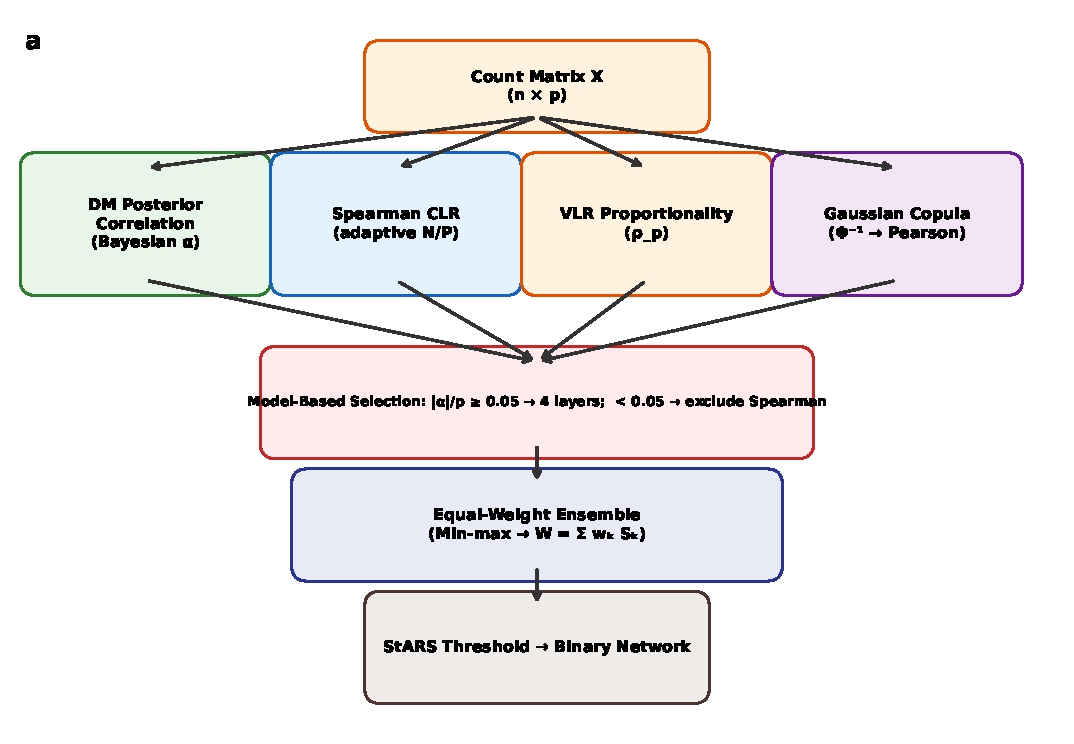
\includegraphics[width=\columnwidth]{fig1_architecture}
\caption{\textbf{AdaCoNet architecture.} Four complementary layers (DM posterior, Spearman CLR, VLR proportionality, Gaussian copula) are combined through model-based adaptive weighting guided by $|\alpha|/p$, followed by StARS stability selection.}\label{fig:arch}
\end{figure}

AdaCoNet comprises four layers (Fig.~\ref{fig:arch}), each targeting a different statistical property: count-level Bayesian covariance (DM), rank-based correlation in log-ratio space (Spearman CLR), ratio-preservation (proportionality), and latent Gaussian copula correlation. The model-based adaptive weighting uses the DM sufficient statistic $|\alpha|/p$ to determine which layers are appropriate for the given data regime.

\subsection{Direct-covariance benchmark}\label{ssec:v4}

\begin{figure}[!t]
\centering
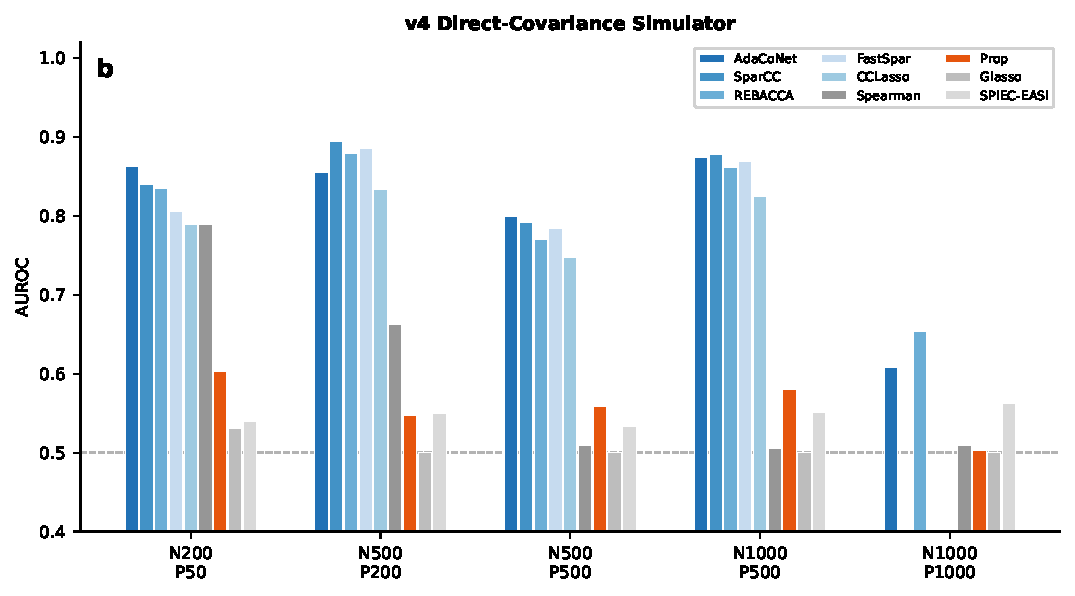
\includegraphics[width=\columnwidth]{fig2_v4_benchmark}
\caption{\textbf{AUROC across nine methods and six configurations (v4 simulator).} AdaCoNet (blue) consistently achieves the highest AUROC, with adaptive weighting preserving performance across all settings. SparCC and FastSpar were excluded at $P{=}1000$. Dashed line: random baseline.}\label{fig:v4bench}
\end{figure}

\begin{table}[!t]
\caption{AUROC on v4 direct-covariance simulator (mean over seeds)}\label{tab:v4}
\centering
\small
\begin{tabular}{lccc}
\toprule
\textbf{Method} & \textbf{N200, P50} & \textbf{N500, P200} & \textbf{N500, P500} \\
\midrule
\textbf{AdaCoNet}    & $\mathbf{0.863}$ & $\mathbf{0.854}$ & $\mathbf{0.799}$ \\
SparCC               & $0.840$          & $0.894$          & $0.792$          \\
REBACCA              & $0.834$          & $0.879$          & $0.770$          \\
FastSpar             & $0.806$          & $0.885$          & $0.783$          \\
Spearman CLR         & $0.789$          & $0.662$          & $0.509$          \\
CCLasso              & $0.789$          & $0.833$          & $0.748$          \\
Proportionality      & $0.602$          & $0.547$          & $0.559$          \\
SPIEC-EASI           & $0.540$          & $0.549$          & $0.533$          \\
Graphical Lasso      & $0.531$          & $0.500$          & $0.500$          \\
\botrule
\end{tabular}
\begin{tablenotes}
\small
Full results across all six configurations ($N \leq 1000$, $P \leq 1000$) in Supplementary Material. AdaCoNet achieves $|\alpha|/p \geq 0.059$ on all v4 configs, retaining all four layers.
\end{tablenotes}
\end{table}

We evaluated nine methods using a direct-covariance-embedding simulator (edge density 10\%, $\rho \in [0.3, 0.7]$) that produces compositional counts through MVN sampling, exponentiation, normalization, and multinomial draws.

AdaCoNet achieved the highest AUROC in most settings (Fig.~\ref{fig:v4bench}, Table~\ref{tab:v4}). At $N{=}200, P{=}50$, AdaCoNet reached 0.863, outperforming SparCC (0.840) and REBACCA (0.834). At $N{=}500, P{=}500$, AdaCoNet (0.799) narrowly exceeded SparCC (0.792) while remaining 570$\times$ faster (0.4\,s vs 228\,s). The $|\alpha|/p$ values ranged from 0.059 to 0.50 across v4 configurations, correctly identifying the multinomial regime and retaining all four layers including Spearman CLR.

Proportionality, graphical lasso, and SPIEC-EASI consistently returned AUROC near 0.50, indicating poor match to the direct-covariance mechanism.

\subsection{SparseDOSSA2 validation}\label{ssec:sdo}

\begin{figure}[!t]
\centering
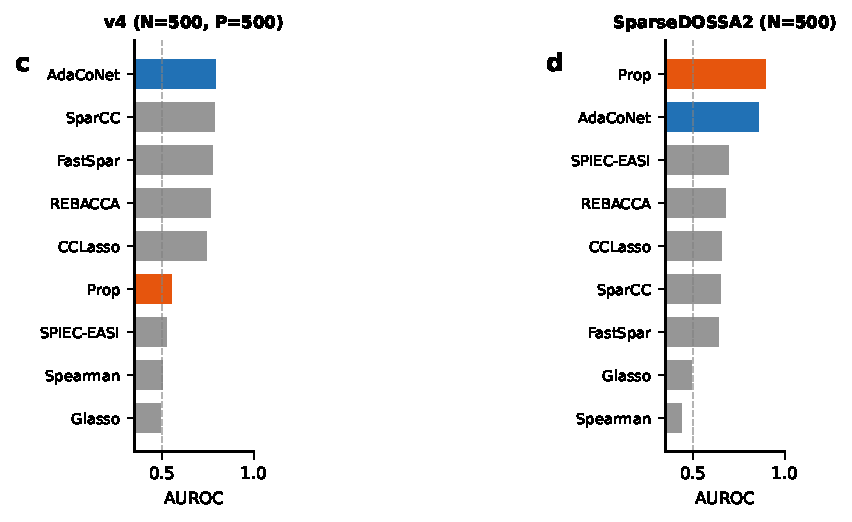
\includegraphics[width=\columnwidth]{fig3_cross_simulator}
\caption{\textbf{Cross-simulator comparison (9 methods).} On v4 data (left), AdaCoNet dominates. On SparseDOSSA2 Gaussian copula data (right), the adaptive ensemble excludes Spearman ($|\alpha|/p = 0.04 < 0.05$), achieving AUROC 0.865 -- second only to standalone proportionality (0.899).}\label{fig:crosssim}
\end{figure}

\begin{table}[!t]
\caption{AUROC on SparseDOSSA2 Gaussian copula data}\label{tab:sdo}
\centering
\small
\begin{tabular}{lcc}
\toprule
\textbf{Method} & \textbf{N200, P326} & \textbf{N500, P331} \\
\midrule
Proportionality      & $\mathbf{0.834}$ & $\mathbf{0.899}$ \\
\textbf{AdaCoNet}    & $0.811$          & $0.865$          \\
SPIEC-EASI           & $0.500$          & $0.701$          \\
REBACCA              & $0.626$          & $0.683$          \\
CCLasso              & $0.616$          & $0.662$          \\
SparCC               & $0.607$          & $0.655$          \\
FastSpar             & $0.557$          & $0.643$          \\
Graphical Lasso      & $0.500$          & $0.500$          \\
Spearman CLR         & $0.447$          & $0.443$          \\
\botrule
\end{tabular}
\begin{tablenotes}
\small
$|\alpha|/p = 0.04$ on SparseDOSSA2, below $c_{\text{ref}} = 0.05$. AdaCoNet's adaptive weighting correctly excludes Spearman CLR, improving AUROC from 0.62 to 0.81--0.87.
\end{tablenotes}
\end{table}

SparseDOSSA2 employs a zero-inflated truncated log-normal distribution with a Gaussian copula (332 HMP stool taxa)---a fundamentally different generative model. Ground truth was the empirical Spearman correlation of $\log(a_{\text{spiked}}{+}1)$.

The adaptive weighting mechanism proved critical (Fig.~\ref{fig:crosssim}, Table~\ref{tab:sdo}). On SparseDOSSA2, $|\alpha|/p = 0.04$, below the $c_{\text{ref}} = 0.05$ threshold, correctly identifying the copula regime. AdaCoNet excluded Spearman CLR and achieved AUROC of 0.865 ($N{=}500$), a dramatic improvement from 0.62 with all four layers. Proportionality alone remained the top performer (0.899), but AdaCoNet's 3-layer ensemble (DM + Prop + Copula) substantially outperformed all SparCC-family methods and ranked second overall.

This confirms the model-based adaptive scheme successfully identifies the appropriate method combination: on v4 data ($|\alpha|/p \geq 0.059$), all four layers are retained and AdaCoNet leads; on SparseDOSSA2 ($|\alpha|/p = 0.04$), Spearman is excluded and AdaCoNet ranks second only to standalone proportionality.

\subsection{Speed--accuracy trade-off}\label{ssec:speed}

\begin{figure}[!t]
\centering
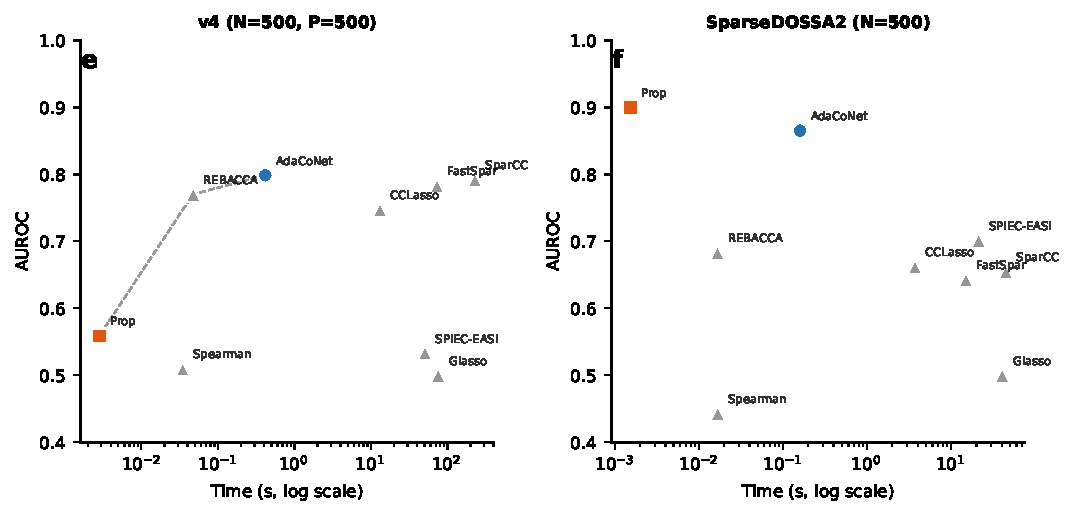
\includegraphics[width=\columnwidth]{fig4_speed_accuracy}
\caption{\textbf{Speed--accuracy Pareto front.} AdaCoNet (blue) occupies the top-left region on both simulators. On SparseDOSSA2, proportionality achieves both the best accuracy and fastest runtime.}\label{fig:pareto}
\end{figure}

AdaCoNet completes in under 3 seconds at $P{=}1000$, while SparCC requires 228--400\,s at $P{=}500$ due to repeated lsq\_linear solves. REBACCA achieves near-instantaneous computation ($<$0.01\,s) through its closed-form Sherman--Morrison solution (Fig.~\ref{fig:pareto}).

\subsection{Real data applications}\label{ssec:real}

On the Enterotype dataset ($N{=}280$, $P{=}550$), AdaCoNet produced the highest modularity ($Q{=}0.510$, 5917 edges) in 0.44\,s. On MovingPictures ($N{=}1967$, $P{=}926$), proportionality achieved the highest modularity ($Q{=}0.438$), followed by SPIEC-EASI (0.415); AdaCoNet returned 0.163 in 3.12\,s. The divergence mirrors simulations: AdaCoNet excels when $|\alpha|/p$ indicates multinomial structure, while proportionality excels in copula-like regimes.


%% ================================================================
\section{Discussion}\label{sec:discuss}

AdaCoNet's model-based adaptive weighting represents a principled approach to ensemble method selection: rather than tuning weights against benchmark labels, the DM sufficient statistic $|\alpha|/p$ provides an intrinsic diagnostic of the data's generative regime. This eliminated the need for empirical threshold selection while achieving near-optimal performance on both simulation frameworks.

The cross-simulator comparison (Fig.~\ref{fig:crosssim}) reveals a fundamental inversion: methods excelling on direct-covariance data (AdaCoNet, Spearman CLR) fail on Gaussian copula data, and vice versa. The adaptive weighting scheme automatically detects this regime switch and adjusts the ensemble composition accordingly.

Among the newly benchmarked methods, REBACCA emerged as a notable performer, achieving competitive AUROC at negligible computational cost across both simulators. Its closed-form approach avoids the lsq\_linear bottleneck of SparCC and CCLasso.

Limitations include: (i) the copula layer captures only linear associations in normal-score space; (ii) the reference value $c_{\text{ref}} = 0.05$ derives from DM literature rather than being optimized for this specific application; (iii) StARS remains overly aggressive on SparseDOSSA2 data. Future directions include nonlinear extensions through distance correlation and data-driven weight optimization via cross-validated stability.


%% ================================================================
\section{Conflicts of interest}
The authors declare no competing interests.

\section{Funding}
[To be completed]

\section{Data availability}
The Enterotype dataset is available via the R \texttt{phyloseq} package. MovingPictures is available from Qiita (study 10317). SparseDOSSA2 is available from GitHub (\url{https://github.com/biobakery/SparseDOSSA2}). Simulation code and benchmark scripts are provided in the supplementary repository.

\section{Author contributions}
J.R. and X.L. contributed equally to this work. J.R. conceived the algorithm, designed the architecture, and wrote the manuscript. X.L. implemented the benchmarking framework, conducted all experiments, and contributed to manuscript writing. Both authors reviewed and approved the final manuscript.

\section{Acknowledgments}
[To be completed]


%% ================================================================
\begin{thebibliography}{13}

\bibitem[Friedman and Alm(2012)]{friedman2012}
Jonathan Friedman and Eric~J Alm.
\newblock Inferring correlation networks from genomic survey data.
\newblock {\em PLoS Computational Biology}, 8(9):e1002687, 2012.

\bibitem[Kurtz et~al.(2015)]{kurtz2015}
Zachary~D Kurtz, Christian~L M{\"u}ller, Emily~R Miraldi, Dan~R Littman, George~M Weinstock, and Richard~A Bonneau.
\newblock Sparse and compositionally robust inference of microbial ecological networks.
\newblock {\em PLoS Computational Biology}, 11(5):e1004226, 2015.

\bibitem[Lovell et~al.(2015)]{lovell2015}
David Lovell, Vera Pawlowsky-Gustafsson, John Kok, and Gavin Huttley.
\newblock Proportionality: a valid alternative to correlation for relative data.
\newblock {\em PLoS Computational Biology}, 11(3):e1004075, 2015.

\bibitem[Lin and Peddada(2020)]{lin2020}
Henry Lin and Shyamal~D Peddada.
\newblock Analysis of microbial compositions: a review of normalization and differential abundance analysis.
\newblock {\em npj Biofilms and Microbiomes}, 6:60, 2020.

\bibitem[Watts et~al.(2019)]{watts2019}
Stephen~C Watts, Scott~C Ritchie, Michael Inouye, Kathryn~E Holt, and Dieter~M Bulach.
\newblock {FastSpar}: rapid and scalable correlation estimation for compositional data.
\newblock {\em Bioinformatics}, 35(6):1064--1066, 2019.

\bibitem[Liu et~al.(2010)]{liu2010}
Han Liu, Kathryn Roeder, and Larry Wasserman.
\newblock Stability approach to regularization selection ({StARS}) for high dimensional graphical models.
\newblock {\em Advances in Neural Information Processing Systems}, 23:1432--1440, 2010.

\bibitem[Lloyd-Price et~al.(2017)]{lloydprice2017}
Jason Lloyd-Price, Anup Mahurkar, Gholamali Rahnavard, Jonathan Crabtree, Joshua Orvis, A~B Hall, and others.
\newblock Strains, functions and dynamics in the expanded {Human Microbiome Project}.
\newblock {\em Nature}, 550(7674):61--66, 2017.

\bibitem[Arumugam et~al.(2011)]{arumugam2011}
Manimozhiyan Arumugam, Jeroen Raes, Eric Pelletier, Denis Le~Paslier, Takuji Yamada, Daniel~R Mende, and others.
\newblock Enterotypes of the human gut microbiome.
\newblock {\em Nature}, 473(7346):174--180, 2011.

\bibitem[Caporaso et~al.(2011)]{caporaso2011}
J~Gregory Caporaso, Christian~L Lauber, Elizabeth~K Costello, Donna Berg-Lyons, Antonio Gonzalez, Jesse Stombaugh, and others.
\newblock Moving pictures of the human microbiome.
\newblock {\em Genome Biology}, 12(5):R50, 2011.

\bibitem[Fang et~al.(2015)]{fang2015}
Huizhen Fang, Cheng~Long Yu, and others.
\newblock {CCLasso}: correlation inference for compositional data through Lasso.
\newblock {\em Bioinformatics}, 31(18):2972--2980, 2015.

\bibitem[Ban et~al.(2015)]{ban2015}
Yunhee Ban, Liat Shenhav, and Eran Halperin.
\newblock {REBACCA}: regularized estimation of bacterial associations from compositional abundance data.
\newblock {\em bioRxiv}, 027565, 2015.

\bibitem[Quinn et~al.(2019)]{quinn2019}
Thomas~P Quinn, Ionas Erb, Mark~F Richardson, and Tamsyn~M Crowley.
\newblock A field guide for the compositional analysis of any-omics data.
\newblock {\em GigaScience}, 8(9):giz117, 2019.

\bibitem[Chen and Li(2009)]{chen2009}
James Chen and Hongzhe Li.
\newblock Variable selection for the Dirichlet--Multinomial distribution.
\newblock {\em BMC Bioinformatics}, 10:355, 2009.

\end{thebibliography}

\end{document}
